% file: 3-9-connectivity/cut-vertex-structure.tex

\documentclass[tikz]{standalone}
\usetikzlibrary{positioning, fit, shapes}

\begin{document}
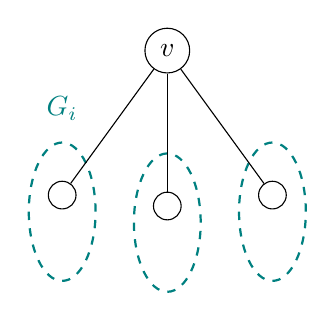
\begin{tikzpicture}[every node/.style = {draw, circle, minimum size = 10pt},
    node distance = 1.5cm and 1.0cm,
    comp/.style = {yshift = -6pt, draw, thick, dashed, teal, ellipse, minimum height = 50pt, minimum width = 18pt}]
  \node (v) {$v$};
  \node (x) [below = of v] {};
  \node (u) [below left = of v] {};
  \node (w) [below right = of v] {};

  \node [fit = (x), comp] {};
  \node [fit = (u), comp, label = {[above, teal] $G_i$}] {};
  \node [fit = (w), comp] {};

  \path (v) edge (x)
  	    edge (u)
	    edge (w);
\end{tikzpicture}
\end{document}
